\documentclass[a4paper]{article}

\setlength{\parindent}{0pt}
\setlength{\parskip}{1em}

\pagestyle{headings}

\usepackage{amssymb}
\usepackage{amsmath}
\usepackage{amsthm}
\usepackage{mathtools}
\usepackage{graphicx}
\usepackage{hyperref}
\usepackage{color}
\usepackage{microtype}
\usepackage{tikz}
\usepackage{pgfplots}
\usepackage{pgfplotstable}

\newcommand{\N}{\mathbb{N}}
\newcommand{\Q}{\mathbb{Q}}
\newcommand{\Z}{\mathbb{Z}}
\newcommand{\R}{\mathbb{R}}
\newcommand{\C}{\mathbb{C}}
\newcommand{\D}{\mathcal{D}}
\renewcommand{\S}{\mathcal{S}}
\renewcommand{\P}{\mathbb{P}}
\newcommand{\F}{\mathbb{F}}
\newcommand{\E}{\mathbb{E}}
\newcommand{\bra}{\langle}
\newcommand{\ket}{\rangle}


\graphicspath{{Image/}}

\hypersetup{
    colorlinks=true,
    linktoc=all,
    linkcolor=blue
}

\theoremstyle{definition}
\newtheorem*{axiom}{Axiom}
\newtheorem*{claim}{Claim}
\newtheorem*{conv}{Convention}
\newtheorem*{coro}{Corollary}
\newtheorem*{defi}{Definition}
\newtheorem*{eg}{Example}
\newtheorem*{lemma}{Lemma}
\newtheorem*{notation}{Notation}
\newtheorem*{prob}{Problem}
\newtheorem*{post}{Postulate}
\newtheorem*{prop}{Proposition}
\newtheorem*{rem}{Remark}
\newtheorem*{thm}{Theorem}

\DeclareMathOperator{\vdiv}{div}
\DeclareMathOperator{\grad}{grad}
\DeclareMathOperator{\curl}{curl}
\DeclareMathOperator{\Ann}{Ann}
\DeclareMathOperator{\Fit}{Fit}
\DeclareMathOperator{\Diag}{Diag}
\DeclareMathOperator{\tr}{tr}
\DeclareMathOperator{\im}{im}
\DeclareMathOperator{\Mat}{Mat}
\DeclareMathOperator{\Log}{Log}
\DeclareMathOperator{\Isom}{Isom}
\DeclareMathOperator{\Mesh}{Mesh}
\DeclareMathOperator{\Sym}{Sym}
\DeclareMathOperator{\Aut}{Aut}
\DeclareMathOperator{\cosech}{cosech}
\DeclareMathOperator{\Card}{Card}
\DeclareMathOperator{\Gal}{Gal}


\setcounter{section}{0}

\begin{document}

\title{Model Theory}

\maketitle

\newpage

\tableofcontents

\newpage

\section{Langauges and structures}

\begin{defi} (1.1)
A language $L$ consists of:\\
$\bullet$(i) a set $\mathcal{F}$ of function symbols, and for each $f \in \mathcal{F}$, a positive integer $n_f$, the arity of $f$;\\
$\bullet$(ii) a set $\mathcal{R}$ of relation symbols, and for each $R \in \mathcal{R}$, a positive integer $n_R$, the arity of $R$;\\
$\bullet$(iii) a set $\mathcal{C}$ of constant symbols.\\
Note that each of the above three sets can be empty.
\end{defi}

\begin{eg}
$L=\{\{\cdot,-1\},\{1\}\}$ where $\cdot$ is a binary function, $-1$ is a unary function, and $1$ is a constant. We call this $L_{gp}$ (language of groups);\\
$L_{lo} = \{<\}$, where $<$ is a binary relation (linear order).
\end{eg}

\begin{defi} (1.2)\\
Given a language $L$, say, an $L$-structure consists of:\\
(i) a set $M$, the \emph{domain};\\
(ii) for each $f \in \mathcal{F}$, a function $f^M:M^{n_f} \to M$;\\
(iii) for each $R \in \mathcal{R}$, a relation $R^M \subseteq M^{n_R}$;\\
(iv) for each $c \in \mathcal{C}$, an element $c^M \in M$.

$f^M,R^M,c^M$ are called the \emph{interpretation} of $f,R,c$ respectively.
\end{defi}

\begin{notation} (1.3)\\
We often fail to distinguish between the symbols in the language $L$ and their interpretations in a $L$-structure, if the context allows.

We may write $\mathcal{M} = \bra M,\mathcal{F},\mathcal{R},\mathcal{C}\ket$.
\end{notation}

\begin{eg} (1.4)\\
(a) $\mathcal{R} = \bra\R^+,\{\cdot,-1\},1\ket$ is an $L_{gp}$-structure.\\
$\mathcal{Z} = \bra\Z,\{+,-\},0\ket$ is also an $L_{gp}$-structure (here $+$ is a binary and $-$ is the unary negation function).\\
$\mathcal{Q} = \bra\Q,<\ket$ is an $L_{lo}$ structure ($<$ is the interpretation of relation).
\end{eg}

\begin{defi} (1.5)\\
Let $L$ be a language, let $\mathcal{M}$ and $\mathcal{N}$ be $L$-structures.\\
An \emph{embedding} of $\mathcal{M}$ into $\mathcal{N}$ is an injection $\alpha:M \to N$ that preserves the structure:\\
(i) For all $f \in \mathcal{F}$, and $a_1,...,a_{n_f} \in M$,
\begin{equation*}
\begin{aligned}
\alpha(f^M(a_1,...,a_{n_f})) = f^N(\alpha(a_1),...,\alpha(a_{n_f}))
\end{aligned}
\end{equation*}
(ii) For all $R \in \mathcal{R}$, and $a_1,...,a_{n_R} \in M$,
\begin{equation*}
\begin{aligned}
(a_1,...,a_{n_R}) \in R^M \iff (\alpha(a_1),...,\alpha(a_{n_R})) \in R^N
\end{aligned}
\end{equation*}
Note that this is an if and only if.\\
(iii) For all $c \in \mathcal{C}$, we need 
\begin{equation*}
\begin{aligned}
\alpha(c^M) = c^N
\end{aligned}
\end{equation*}
As anyone could expect, a surjective embedding $\mathcal{M} \to \mathcal{N}$ is also called an \emph{isomorphism} of $\mathcal{M}$ onto $\mathcal{N}$.
\end{defi}

(1.6) Exercise. Let $G_1,G_2$ be groups, regarded as $L_{gp}$-structures.\\
Check that $G_1 \cong G_2$ in the usual algebra sense, if and only if there is an isomprhism $\alpha:G_1\ \to G_2$ in the sense of above definition 1.5.

\newpage

\section{Terms, formulae, and their interpretations}
In addition to the symbols of $L$, we also have:\\
(i) infinitely many variables, $\{x_i\}_{i \in I}$;\\
(ii) logical connectives, $\wedge,\neg$ (also express $\vee, \to, \leftrightarrow$);\\
(iii) quantifier $\exists$ (also express $\forall$);\\
(iv) punctuations $(,)$.

\begin{defi} (2.1) \\
\emph{$L$-terms} are defined recursively as follows:\\
$\bullet$ any variable $x_i$ is a term;\\
$\bullet$ any constant symbol is a term;\\
$\bullet$ for any $f \in \mathcal{F}$, 
\begin{equation*}
\begin{aligned}
f(t_1,...,t_{n_f})
\end{aligned}
\end{equation*}
for any terms $t_1,...,t_{n_f}$ is a term;\\
$\bullet$ nothing else is a term.
\end{defi}

Notation: we write $t(x_1,...,x_n)$ to mean that the variables appearing in $t$ are among $x_1,..,x_n$.

\begin{eg}
In $\mathcal{R} = <\R,\cdot,-1,1>$,\\
$\bullet$ $(\cdot (x_1,x_2),x_3)$ is a term ($x_1 \cdot x_2) \cdot x_3$);\\
$\bullet$ $(\cdot (1,x_1))^{-1}$ is a term ($1 \cdot x)^{-1}$.
\end{eg}

\begin{defi} (2.2)\\
If $\mathcal{M}$ is an $L$-structure, to each $L$-term $t(x_1,...,x_k)$ we assign a function
\begin{equation*}
\begin{aligned}
t^M: M^k \to M
\end{aligned}
\end{equation*}
defined as follows:\\
(i) If $t = x_i, t^M [a_1,...,a_k] = a_i$;\\
(ii) If $t=c$ is a constant, $t^M [a_1,...,a_k] = c^m$;\\
(iii) If $t=f(t_1(x_1,...,x_k),...,t_{n_f}(x_1,...,x_k))$, 
\begin{equation*}
\begin{aligned}
t^M (a_1,...,a_k) = f^M(t_1^M(a_1,...,a_k),...,t_{n_f}^M(a_1,...,a_k))
\end{aligned}
\end{equation*}
\end{defi} 

---Lecture 2---

No lecture this friday (12th Oct)! Will have an extra one on Monday 22 Oct at 12 (MR12).

First example class: Monday 29th Oct at 12.

Info on course and notes on $http:\\users.mct.open.ac.uk/sb27627/MT.html$ (it seems that it only comes after lecture, and is hand-written, so this notes still continues), or google \emph{Silvia Barbina MCT} and follow link \emph{Part III Model Theory} on lecturer's homepage.

\begin{rem}
    (The lecture forgot about this last time) Any language $L$ includes an equality symbol $=$.
\end{rem}

Last time we assigned a function $t^m$. In $L_{gp}$, the term $x_2 \cdot x_3$ can be described as, say $t_1(x_1,x_2,x_3),t_2(x_1,x_2,x_3,x_4),...$.\\
Then the term $x_2 \cdot x_3$ can be assigned to functions $t_1^M:M^3\to M:(a_1,a_2,a_3) \to (a_2 \cdot a_3)$, or $t_2^M: M^4 \to M: (a_1,a_2,a_3,a_4) \to (a_2 \cdot a_3)$. These syntactic things are not really important -- we just have to know that there is a corresponding action for each term.

We now define the \emph{complexity} of a term $t$ to be the number of symbols of $L$ occuring in $t$.

Fact (2.3): Let $\mathcal{M}$ and $\mathcal{N}$ be $L$-structures, and let $\alpha:\mathcal{M} \to \mathcal{N}$ be an embedding. For any $L$-term $t(x_1,...,x_k)$ and $a_1,...,a_k \in M$, we have
\begin{equation*}
    \begin{aligned}
        \alpha(t^M(a_1,...,a_k)) = t^N(\alpha(a_1),...,\alpha(a_k))
    \end{aligned}
\end{equation*}
\begin{proof}
Prove by induction on complexity of $t$.\\
Let $\bar{a} = (a_1,...,a_k)$ and $\bar{x} = (x_1,...,x_l)$. Then:\\
(i) if $t=x_i$a a variable, then $t^M(\bar{a}) = a_i$, and $t^N(\alpha(a_1),...,\alpha(a_k)) = \alpha(a_i)$, so the conclusion holds;\\
(ii) if $t=c$ is a constant, then $t^M(\bar{a}) = c^M$, and $t^N(\alpha(\bar{a})) = c^N$ by definition of a term. The key here is that, since $\alpha$ is an embedding we have $\alpha(c^M) = c^N$;\\
(iii) if $t = f(t_1(\bar{x},...,t_{n_f}(\bar{x})))$, then
\begin{equation*}
    \begin{aligned}
    \alpha(f^M(t_1^M(\bar{a}),...,t_{n_f}(\bar{a}))) &= f^N(\alpha (t_1^M(\bar{a})),...,\alpha(t_{n_f}^M(\bar{a})))
    \end{aligned}
\end{equation*}
as $\alpha$ is an embedding. But $t_1(\bar{x}),...,t_{n_f}(\bar{x})$ have lower complexity than $t$, so the inductive hypothesis applies.
\end{proof}

Exercise (2.4): conclude the proof of the above fact.\\
(Actually is it not done?)

\begin{defi} (2.5)\\
    The set of \emph{atmoic formulas} of $L$ is defined as follows:\\
    (i) if $t_1,t_2$ are $L$-terms, then $t_1 = t_2$ is an atomic formula;\\
    (ii) if $R$ is a relation symbol, and $t_1,...,t_{n_R}$ are $L$-terms, then $R(t_1,...,t_{n_R})$ is an atomic formula;\\
    (iii) nothing else is an atomic formula.
\end{defi}

\begin{defi} (2.6)\\
    The set of $L$-formulas is defined as follows:\\
    (i) any atomic formula is an $L$-formula;\\
    (ii) if $\phi$ is an $L$-formula, then so is $\neg \phi$;\\
    (iii) if $\phi$ and $\psi$ are $L$-formulas, then so is $\phi \wedge \psi$;\\
    (iv) if $\phi$ is an $L$-formula, for any $i \geq 1$, $\exists x_i \phi$ is a formula;\\
    (v) nothing else is a formula (note that $\forall$ can be constructed by $\neg$ and $\exists$).
\end{defi}

\begin{eg}
    In $L_{gp}$, $x_1\cdot x_1 = x_2$, or $x_1\cdot x_2=1$ are both atomic formulas;\\
    $\exists x_1(x_1 \cdot x_2) = 1$ is an $L$-formula, but (obviously) not atomic.
\end{eg}

A variable occurs \emph{freely} in a formula if it does not occur within the scope of a quantifier $\exists$. We sometimes also say that the variable is \emph{free} (from Part II Logic and Sets). Otherwise we say the variable is \emph{bound}.

We'll use the convention that no variable occurs both freely and as a bound variable in the same formula.

A \emph{sentence} is a formula with no free variables. For example, $\exists x_1\exists x_2 (x_1\cdot x_2=1)$ is an $L_{gp}$-sentence.

Notation: $\phi(x_1,...,x_k)$ means that the free variables in $\phi$ are among $x_1,...,x_k$.

Now we introduce a long and inductive (and also in logic and sets) definition for which sentences are \emph{true}:
\begin{defi} (2.7)\\
    Let $\phi(x_1,...,x_k)$ be an $L$-formula, let $\mathcal{M}$ be an $L$-structure, and let $\bar{a} = a_1,...,a_k$ be elements of $\mathcal{M}$.\\
    We define $\mathcal{M} \vDash \phi(\bar{a})$ (syntactic implication, read as \emph{M models $\phi(\bar{a})$}) as follows:\\
    (i) if $\phi$ is $t_1=t_2$, then $\mathcal{M} \vDash \phi(\bar{a}) \iff t_1^M(\bar{a}) = t_2^M(\bar{a})$;\\
    (ii) if $\phi$ is $R(t_1,...,t_{n_R})$, then $\mathcal{M} \vDash \phi(\bar{a})$ iff
    \begin{equation*}
        \begin{aligned}
            \left(t_1^M(\bar{a}),...,t_{n_R}^M(\bar{a})\right) \in R^M
        \end{aligned}
    \end{equation*}
    (iii) if $\phi$ is a conjunction, say $\psi \wedge \chi$, then $\mathcal{M} \vDash \phi(\bar{a})$ iff $\mathcal{M} \vDash \psi(\bar{a})$ and $\mathcal{M} \vDash \chi(\bar{a})$;\\
    (iv) if $\phi$ is $\exists x_j \chi(x_1,...,x_k,x_j)$ (where we'll assume that $x_j$ is not one of the free variables $x_1,...,x_k$), then $\mathcal{M} \vDash \phi(\bar{a})$ iff there exists $b \in \mathcal{M}$ s.t. $\mathcal{M} \vDash \chi(a_1,...,a_k,b)$;\\
    (v) (lecture forgets this, this should probably be more in front rather than in the end) if $\phi$ is $\neg \psi$, then $\mathcal{M} \vDash \phi(\bar{a})$ iff $\mathcal{M} \not\vDash \psi(\bar{a})$.
\end{defi}

\begin{eg}
    Consider $\mathcal{R} = \bra \R^*,\cdot ,-1,1\ket$, the multiplicative group of non-negative reals, and suppose we have $\phi(x_1) = \exists x_2 (x_2 \cdot x_2 = x_1)$, then $\mathcal{R} \vDash \phi(1)$, but $\mathcal{R} \not\vDash \phi(-1)$.
\end{eg}

Notation (2.8) (useful abbreviations, closer to real life. The precise formulas are not that important -- the abbreviations mean what we expect in real life):\\
$\bullet$ $\phi \vee \psi$ for $\neg(\neg\phi \wedge \neg \psi)$;\\
$\bullet$ $\phi \to \psi$ for $\neg \phi \vee \psi$;\\
$\bullet$ $\phi \leftrightarrow \psi$ for $(\phi \to \psi) \wedge (\psi \to \phi)$;\\
$\bullet$ $\forall x_i \phi$ for $\neg \exists x_i (\neg \phi)$.

\begin{prop} (2.9)\\
    Let $\mathcal{M}$ and $\mathcal{N}$ be $L$-structures, and let $\alpha: \mathcal{M} \to \mathcal{N}$ be an embedding.\\
    Let $\phi(\bar{x})$ be an atomic(!) formula, and $\bar{a} \in M^{|\bar{x}|}$, here $|\bar{x}|$ means the length of the tuple $\bar{x}$ (from now on, when we write a tuple like $\bar{a}$, we will assume that it has the correct length without explicitly stating that), then
    \begin{equation*}
        \begin{aligned}
            \mathcal{M} \vDash \phi(\bar{a}) \iff \mathcal{N} \vDash \phi(\alpha(\bar{a}))
        \end{aligned}
    \end{equation*}
\end{prop}

Question: if $\phi$ is an $L$-formula, not necessarily atomic, does (2.9) still hold? (the answer is no!)

---Lecture 3---

Lecturer wants to reiterate that her email address is $silvia.barbina@open.ac.uk$.\\
Just bring the work along. Unfortunately lecturer doesn't have an office here, so no pigeonhole.\\
Check website for example sheet 1!

Additional assumption: assume the set of variables in a language are indexed by a linearly ordered set.\\
In definition 2.7 we defined what it means for $\mathcal{M} \vDash\phi(\bar{a})$, in particular we defined: if $\phi \equiv \neg \chi$, then $\mathcal{M} \vDash \phi(\bar{a})$ iff $\mathcal{M} \not\vDash \chi(\bar{a})$. Here by $\mathcal{M} \vDash \phi(\bar{a})$ we mean $\mathcal{M} \vDash \neg\chi(\bar{a})$, and $\chi(\bar{a})$ is \emph{shorter} than $\phi(\bar{a})$, so this definition by induction works.

Now let's go back to a sketch proof of (2.9).
\begin{proof}
    There are two cases:\\
    $\bullet$ $\phi(\bar{x})$ is of the form $t_1(\bar{x}) = t_2(\bar{x})$ where $t_1,t_2$ are terms. Use Fact (2.3). (exercise on example sheet)\\
    $\bullet$ $\phi(\bar{x})$ is of the form $R(t_1(\bar{x}),...,t_{n_R} (\bar{x}))$. Then $\mathcal{M} \vDash R(t_1(\bar{a}),...,t_{n_R}(\bar{a}))$ if and only if ... (lecturer says work this out by yourself. Basically the induction step).
\end{proof}

\begin{prop} (2.10)\\
    Exercise: show that prop (2.9) holds if $\phi(\bar{x})$ is a formula without quantifiers (a quantifier-free formula).\\
    (I guess that also suggests when does it not hold for general formulas -- see below).
\end{prop}

\begin{eg} (2.11, Do embeddings preserve all formulas? No.)\\
Let $\mathcal{Z} = (\Z,<)$ an $L_{lo}-$structure, $\mathcal{Q}=(\Q,<)$ also an $L_{lo}-$structure. Then
\begin{equation*}
    \begin{aligned}
        \alpha: &\Z \to \Q\\
        &n \to n
    \end{aligned}
\end{equation*}
is an embedding (check). But:
\begin{equation*}
    \begin{aligned}
        \phi(x_1,x_2) \equiv \exists x_3(x_1<x_3 \wedge x_3 < x_2)
    \end{aligned}
\end{equation*}
Now $\mathcal{Q} \vDash \phi(1,2)$ but $\mathcal{Z} \not\vDash \phi(1,2)$.
\end{eg}

Fact (2.12) (From now on we'll stop saying that $\mathcal{M},\mathcal{N}$ are $L$-structures etc to save time) Let $\alpha: \mathcal{M} \to \mathcal{N}$ be an isomorphism. Then if $\phi(\bar{x})$ is an $L$-formula, and $\bar{a} \in M^{|\bar{x}|}$, then
\begin{equation*}
    \begin{aligned}
        \mathcal{M} \vDash \phi(\bar{a}) \iff \mathcal{N} \vDash \phi(\alpha(\bar{a}))
    \end{aligned}
\end{equation*}
The proof is left as an exercise (another one).

\newpage

\section{Theories and Elementarity}

This is where the core materials begin.

Throughout this chapter, let $L$ be a language, $\mathcal{M},\mathcal{N}$ be $L$-structures.

\begin{defi} (3.1)\\
    An \emph{$L$-theory} $T$ is a set of $L$-sentences.\\
    $\mathcal{M}$ is a \emph{model} of $T$ if $\mathcal{M} \vDash \sigma$ for all $\sigma \in T$. We write $\mathcal{M} \vDash T$.\\
    The class of all the models of $T$ is written $Mod(T)$.\\
    The \emph{theory of $\mathcal{M}$} is the set 
    \begin{equation*}
        \begin{aligned}
            Th(\mathcal{M}) = \{\sigma:\sigma \text{ is an } L-\text{sentence and } \mathcal{M} \vDash \sigma\}
        \end{aligned}
    \end{equation*}
\end{defi}

\begin{eg} (3.2)\\
    Let $T_{gp}$ be the set of $L_{gp}$-sentences:\\
    (i) $\forall x_1x_2x_3 (x_1 \cdot (x_2 \cdot x_3) = (x_1\cdot x_2) \cdot x_3)$;\\
    (ii) $\forall x_1 (x_1 \cdot 1 = 1 \cdot x_1 = x_1)$;\\
    (iii) $\forall x_1 (x_1 \cdot x_1^{-1} = x_1^{-1} \cdot x_1 = 1)$.\\
    Clearly, for a group $G$, $G \vDash T_{gp}$ (as they are just the group axioms). However, for a specific group $G$, clearly the theory of it, $Th(G)$ is lartger than $T_{gp}$.
\end{eg}

\begin{defi} (3.3)\\
    $\mathcal{M}$ and $\mathcal{N}$ are \emph{elementarily equivalent} if $Th(\mathcal{M}) = Th(\mathcal{N})$.\\
    We write $\mathcal{M} \equiv \mathcal{N}$.\\
    Clearly, if $\mathcal{M} \simeq \mathcal{N}$ ($\simeq$ means isomorphism), then $\mathcal{M} \equiv \mathcal{N}$.\\
    But if $\mathcal{M}$ and $\mathcal{N}$ are not isomorphic, establishing whether $\mathcal{M} \equiv \mathcal{N}$ can be highly non-trivial!\\
    We'll see $(\Q,<) \equiv (\R,<)$ as $L_{lo}-$structures(!).
\end{defi}

\begin{defi} (3.4)\\
    (i) An embedding $\beta: \mathcal{M} \to \mathcal{N}$ is \emph{elementary} if for all formulas $\phi(\bar{x})$ and $\bar{a} \in M^{|\bar{x}|}$,
    \begin{equation*}
        \begin{aligned}
            \mathcal{M} \vDash \phi(\bar{a}) \iff \mathcal{N} \vDash \phi(\beta(\bar{a}))
        \end{aligned}
    \end{equation*}
    (ii) If $M \subseteq N$, and $id:\mathcal{M} \to \mathcal{N}$ is an embedding, then $\mathcal{M}$ is a \emph{substructure} of $\mathcal{N}$.\\
    (iii) If $M \subseteq N$ and $id:\mathcal{M} \to \mathcal{N}$ is an \emph{elementary embedding} (just accept it without thinking of what it actually means in reality), then $\mathcal{M}$ is said to be an \emph{elementary substructure} of $\mathcal{N}$, written as $\mathcal{M} \preccurlyeq \mathcal{N}$.
\end{defi}

\begin{eg} (3.5)\\
    Let $\mathcal{M} = [0,1] \subseteq \R$, an $L_{lo}-$structure where $<$ is the usual order;\\
    Let $\mathcal{N} = [0,2] \subseteq \R$, also an $L_{lo}-$structure with the same $<$.\\
    Then $\mathcal{M} \simeq \mathcal{N}$ as $L_{lo}-$structures. So $\mathcal{M} \equiv \mathcal{N}$ (since they are isomoprhic).\\
    Also, $\mathcal{M} \subseteq \mathcal{N}$ (read as \emph{is a substructure of}), since the ordering $<$ coincides on $\mathcal{M}$ and $\mathcal{N}$. \emph{However}, $\mathcal{M} \not\preccurlyeq \mathcal{N}$, since if we pick the formula $\phi(x) \equiv \exists y (x<y)$, then $\mathcal{N} \vDash \phi(1)$, but $\mathcal{M} \not\vDash \phi(1)$.
\end{eg}

\begin{defi} (3.6)\\
    Let $\mathcal{M}$ be an $L$-structure, $A \subseteq M$, then
    \begin{equation*}
        \begin{aligned}
            L(A) = L \cup \{c_a:a \in A\}
        \end{aligned}
    \end{equation*}
    (where $c_a$ are constant symbols). An interpretation of $\mathcal{M}$ as an $L$-structure extends to an interpretation of $\mathcal{M}$ as an $L(A)$-structure in the obvious way, i.e. $c_a^M = a$.\\
    In this context, the elements of $A$ are called \emph{parameters}.\\
    If $\mathcal{M}$ and $\mathcal{N}$ are two structures, and $A \subseteq M \cap N$, then
    \begin{equation*}
        \begin{aligned}
            \mathcal{M} \equiv_A \mathcal{N}
        \end{aligned}
    \end{equation*}
    where we mean $\mathcal{M},\mathcal{N}$ satisfy exactly the same $L(A)$ sentences.
\end{defi}

---Lecture 4---

Reminder: we have a lecture next Monday (22nd Oct)!

\begin{prop}
    It turns out that, $\mathcal{M} \preccurlyeq \mathcal{N} \iff \mathcal{M} \equiv_M \mathcal{N}$ (where $M$ is the domain of $\mathcal{M}$).
\end{prop}

\begin{lemma} (3.8, Tarski-Vaught test)\\
    Let $\mathcal{N}$ be an $L$-structure, let $A \subseteq N$. The follwing are equivalent:\\
    (i) $A$ is the domain of a structure $\mathcal{M}$ s.t. $\mathcal{M} \preccurlyeq \mathcal{N}$;\\
    (ii) if $\phi(x) \in L(A)$ (with an abuse of notations $\phi(x,c_{a_1},...,c_{a_n}) = \phi(x,a_1,...,a_n)$), if $\mathcal{N} \vDash \exists x \phi(x)$, then $\mathcal{N} \vDash \phi(b)$ for some $b \in A$.
    \begin{proof}
        (i) $\implies$ (ii): Suppose $\mathcal{N} \vDash \exists x \phi(x)$. Then by elementarity, $\mathcal{M} \vDash \exists x \phi(x)$, and so $\mathcal{M} \vDash \phi(b)$ for $b \in \mathcal{M}$. So (again by elementarity), $\mathcal{N} \vDash \phi(b)$.\\
        (ii) $\implies$ (i): This is the harder direction. First we prove that $A$ is the domain of a substructure $\mathcal{M} \subseteq \mathcal{N}$.\\
        By Sheet 1 Q4, it suffices to check:\\
        (a) For each constant $c$, $c^N \in A$;\\
        (b) For each function symbol $f$, $f^N(\bar{a}) \in A$ (for all $\bar{a} \in A^{n_R}$);\\
        For (a), use property (ii) with $\exists x (x=c)$.\\
        For (b), use property (ii) with the formula $\exists x ((\bar{a}) = x)$.\\
        So we now have $\mathcal{M} \subseteq \mathcal{N}$, and domain of $\mathcal{M}$ is $A$. But we actually want to prove that $\mathcal{M} \preccurlyeq \mathcal{N}$. Now let $\chi(\bar{x})$ be an $L$-formula.\\
        We want to show that for $\bar{a} \in A^{|\bar{x}|}$ $\mathcal{M} \vDash \chi(\bar{a}) \iff \mathcal{N} \vDash \chi(\bar{a})$ (*).\\
        By induction on the complexity of $\chi(\bar{x})$:\\
        $\bullet$ if $\chi(\bar{x})$ is atomic, (*) follows from $\mathcal{M} \subseteq \mathcal{N}$ (since $\mathcal{M}$ is a substructure!);\\
        $\bullet$ if $\chi(\bar{x})$ is $\neg \psi(\bar{x})$ or $\chi(\bar{x})$ is $\psi(\bar{x})\wedge \xi(\bar{x})$, it's a straightforward induction;\\
        $\bullet$ (interesting case) if $\chi(\bar{x}) = \exists y \psi(\bar{x},y)$ where $\psi(\bar{x},y)$ is an $L$-formula, suppose that $\mathcal{M} \vDash \chi(\bar{a})$, then $\mathcal{M} \vDash \exists y \psi(\bar{a},y)$, hence $\mathcal{M} \vDash \psi(\bar{a},b)$ for some $b \in A = \dom (\mathcal{M})$ (this is the definition of truth).\\
        But then $\mathcal{N} \vDash \psi(\bar{a},b)$ by inductive hypothesis, so $\mathcal{N} \vDash \chi(\bar{a})$.\\
        Now let $\mathcal{N} \vDash \chi(\bar{a})$, i.e. $\mathcal{N} \vDash \exists y \psi (\bar{a},y)$ (we find a \emph{witness} for it). By property (ii), $\mathcal{N} \vDash \psi(\bar{a},b)$ for some $b \in A = \dom(\mathcal{M})$.\\
        Again by inductive hypothesis, we have $\mathcal{M} \vDash \psi(\bar{a},b)$, and so in particular, $\mathcal{M} \vDash \chi(\bar{a})$ as it has got a witness there.
    \end{proof}
\end{lemma}

\begin{rem} (3.9)\\
    Even more assumptions: let's assume that the set of variables is countably infinite. Then:\\
    $\bullet$ the cardinality of the set of $L$-formulas is $|L|+\omega$ (where by $|L|$ we mean the number of symbols. For example, $|L_{gp}| = 3$, $|L_{lo}| = 1$), where we abuse another notation that we use $\omega$ as cardinals (rather than ordinals) (note that the formulas are just strings of finite length);\\
    $\bullet$ if $A$ is a set of parameters in some structure, the cardinality of the set $L(A)$ is $|A|+|L|+\omega$, where by $+$ here we merely mean $\max\{|L|,|A|,\omega\}$ (instead of addition), and same for the $+$ above.
\end{rem}

\begin{defi} (3.10)\\
    Let $\lambda$ be an ordinal. Then \emph{a chain of length} $\lambda$ of sets is a sequence $\bra M_i : i < \lambda \ket$, where $M_i \subseteq M_j$ for all $i \leq j < \lambda$.\\
    A chain of $L$-structures is a seequence: $\bra \mathcal{M}_i: i < \lambda \ket$ s.t. $\mathcal{M}_i \subseteq \mathcal{M}_j$ (note that it's substructure here) for $i \leq j < \lambda$.\\
    The \emph{union} of this chain is the $L$-structure $\mathcal{M}$ defined as follows:\\
    $\bullet$ the domain is $\bigcup_{i<\lambda} M_i$ (when you think of this, you can always start with the case $\lambda = \omega$);\\
    $\bullet$ for constants $c$, $c^M = c^{M_i}$ for any $i<\lambda$ (this is well defined, because of the substructure condition above);\\
    $\bullet$ if $f$ is a function symbol, $\bar{a} \in M^{|n_f|}$ (why the mod sign here), $f^M \bar{a} = f^{M_i} \bar{a}$ where $i$ is s.t. $\bar{a} \in M_i^{|n_f|}$;\\
    $\bullet$ if $R$ is a relation synbol, then $R^M = \bigcup_{i < \lambda} R^{M_i}$.
\end{defi}

\begin{thm} (3.11, Downward L$\ddot{o}$wenheim-Skolem theorem)\\
    (Recall that in part II Logic and Set Theory we had the countable version of this)\\
    Let $\mathcal{N}$ be an $L$-structure, and $|\mathcal{N}| \geq |L| + \omega$. Let $A \subseteq N$. Then for every cardinal $\lambda$ s.t. $|L|+|A|+\omega \leq \lambda \leq |\mathcal{N}|$, there is $\mathcal{M} \preccurlyeq \mathcal{N}$ s.t.\\
    (i) $A \subseteq M$;\\
    (ii) $|\mathcal{M}| = \lambda$.

    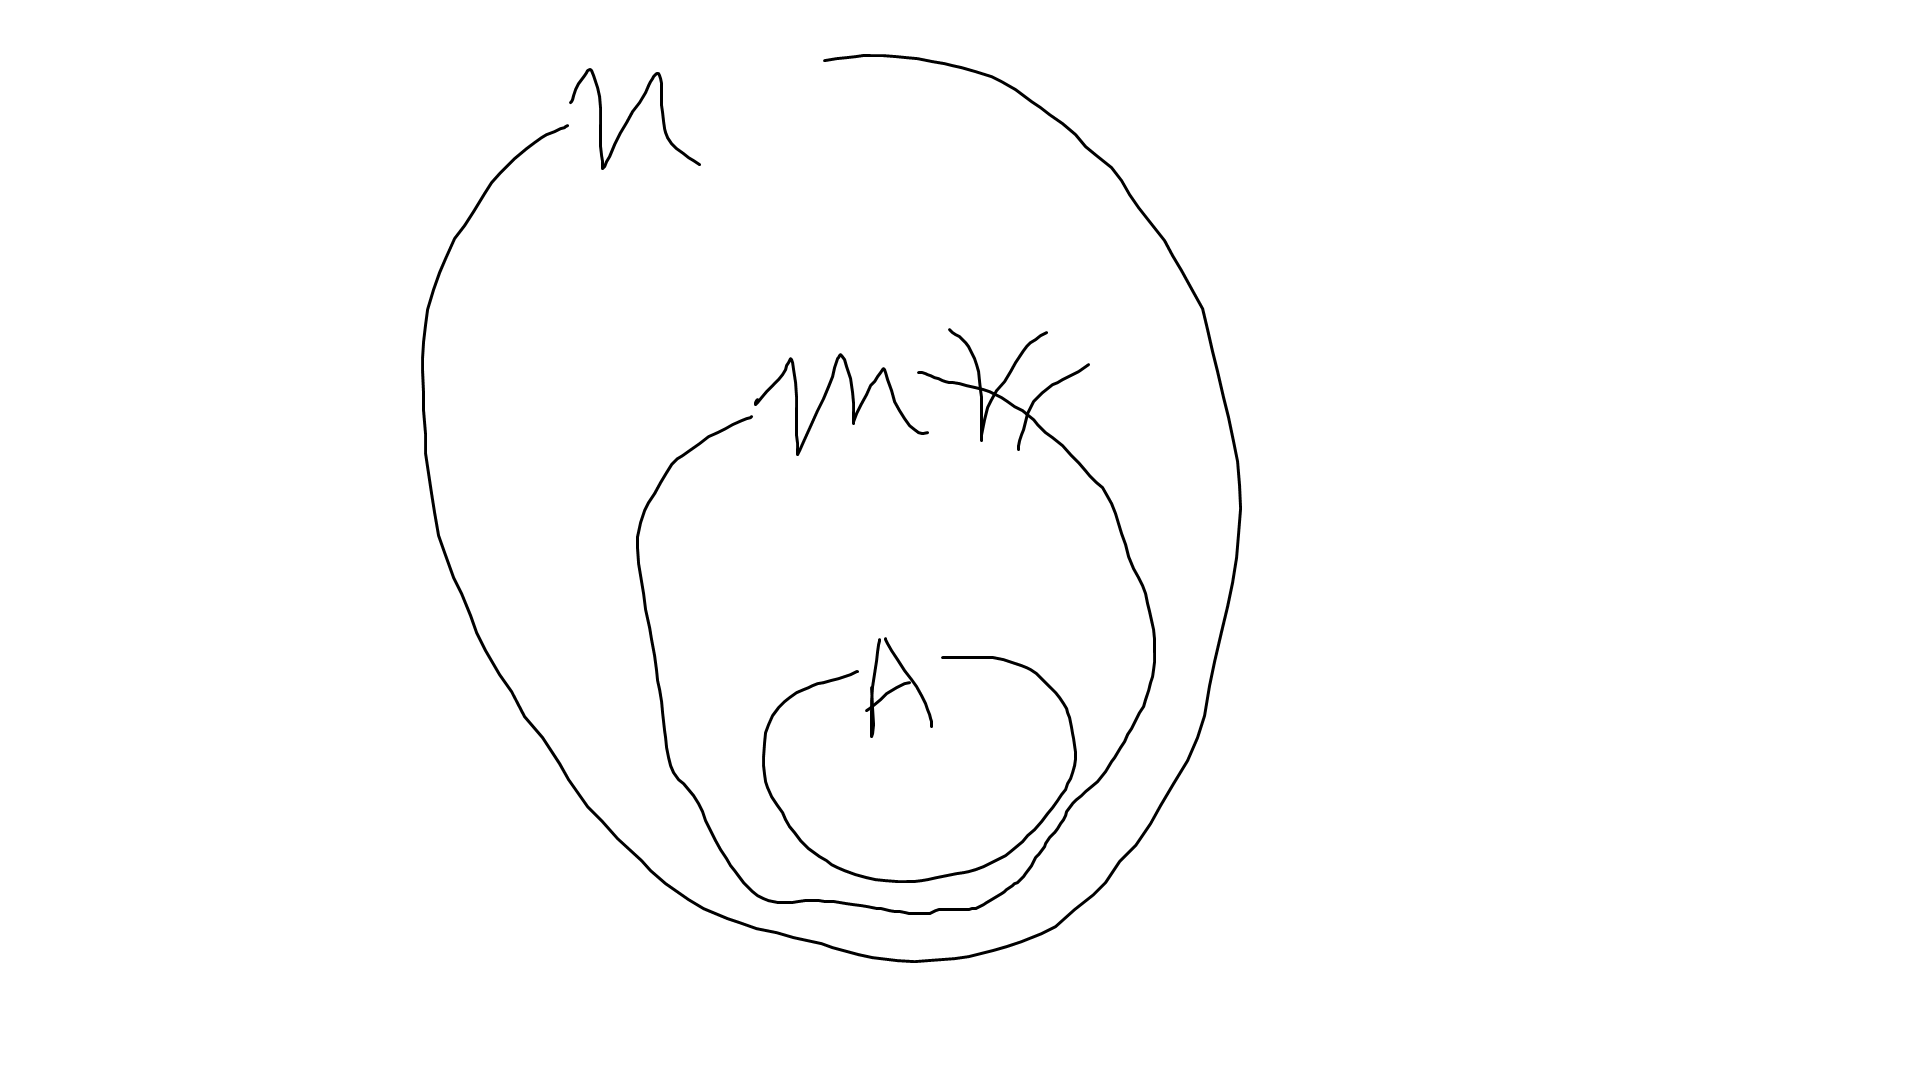
\includegraphics[scale=0.5]{image/Model_01.png}

    (It helps to think about the case $|A| = \omega$ and $|N|$ is uncountable.)\\
    A quick example how this could be useful (we'll go very sloppy here): think of $(\C,+,\cdot,-,\cdot^{-1},0,1)$ as a field. Consider $\Q \subseteq \C$ (both as subset and substructure). Note that algebraic closeness is a property of $\C$. By downward L$\ddot{o}$wenheim-Skolem, there is a substructure in $\mathcal{C}$ that contains $\Q$ that is also algebraically closed (apparently, the set of algebraic numbers).
    \begin{proof}
        We build a chain $\bra A_i : i < \lambda \ket$, with $A_i \subseteq N$, s.t. $|A_i| = \lambda$.\\
        (our goal: define an elementary substructure with domain $M=\bigcup_{i < \omega} A_i$).\\
        Base case: Let $A_0 \subseteq N$ be such that $A \subseteq A_0$ and $|A_0| = \lambda$.\\
        Successors: At stage $i+1$, assume $A_i$ has been built, with $|A_i| = \lambda$.\\
        Let $\bra \phi_k(x): k < \lambda \ket$ be an enumeration of those $L(A_i)$-formulas such that $\mathcal{N} \vDash \exists x \phi_k(x)$. Let $a_k$ be such that $\mathcal{N} \vDash \phi_k(a_k)$, and let $A_{i+1} = A_i \cup \{a_k: k < \lambda\}$ (basically, with those witnesses added). Then $|A_{i+1}| = \lambda$ (note that we haven't increased the size).\\
        Now let $M = \bigcup_{i < \omega} A_i$ (note the subscript range). We use lemma (3.8) to show that $M$ is the domain of $\mathcal{M} \preccurlyeq \mathcal{N}$, and $|M| = \lambda$.
        We're running out of time, so we'll continue next Monday.\\
        
        ---Lecture 5---\\
        Solutions to worksheet 1: either take along to lecture on Friday, or email them to $silvia.barbina@open.ac.uk$.

        Let's continue with the proof:

        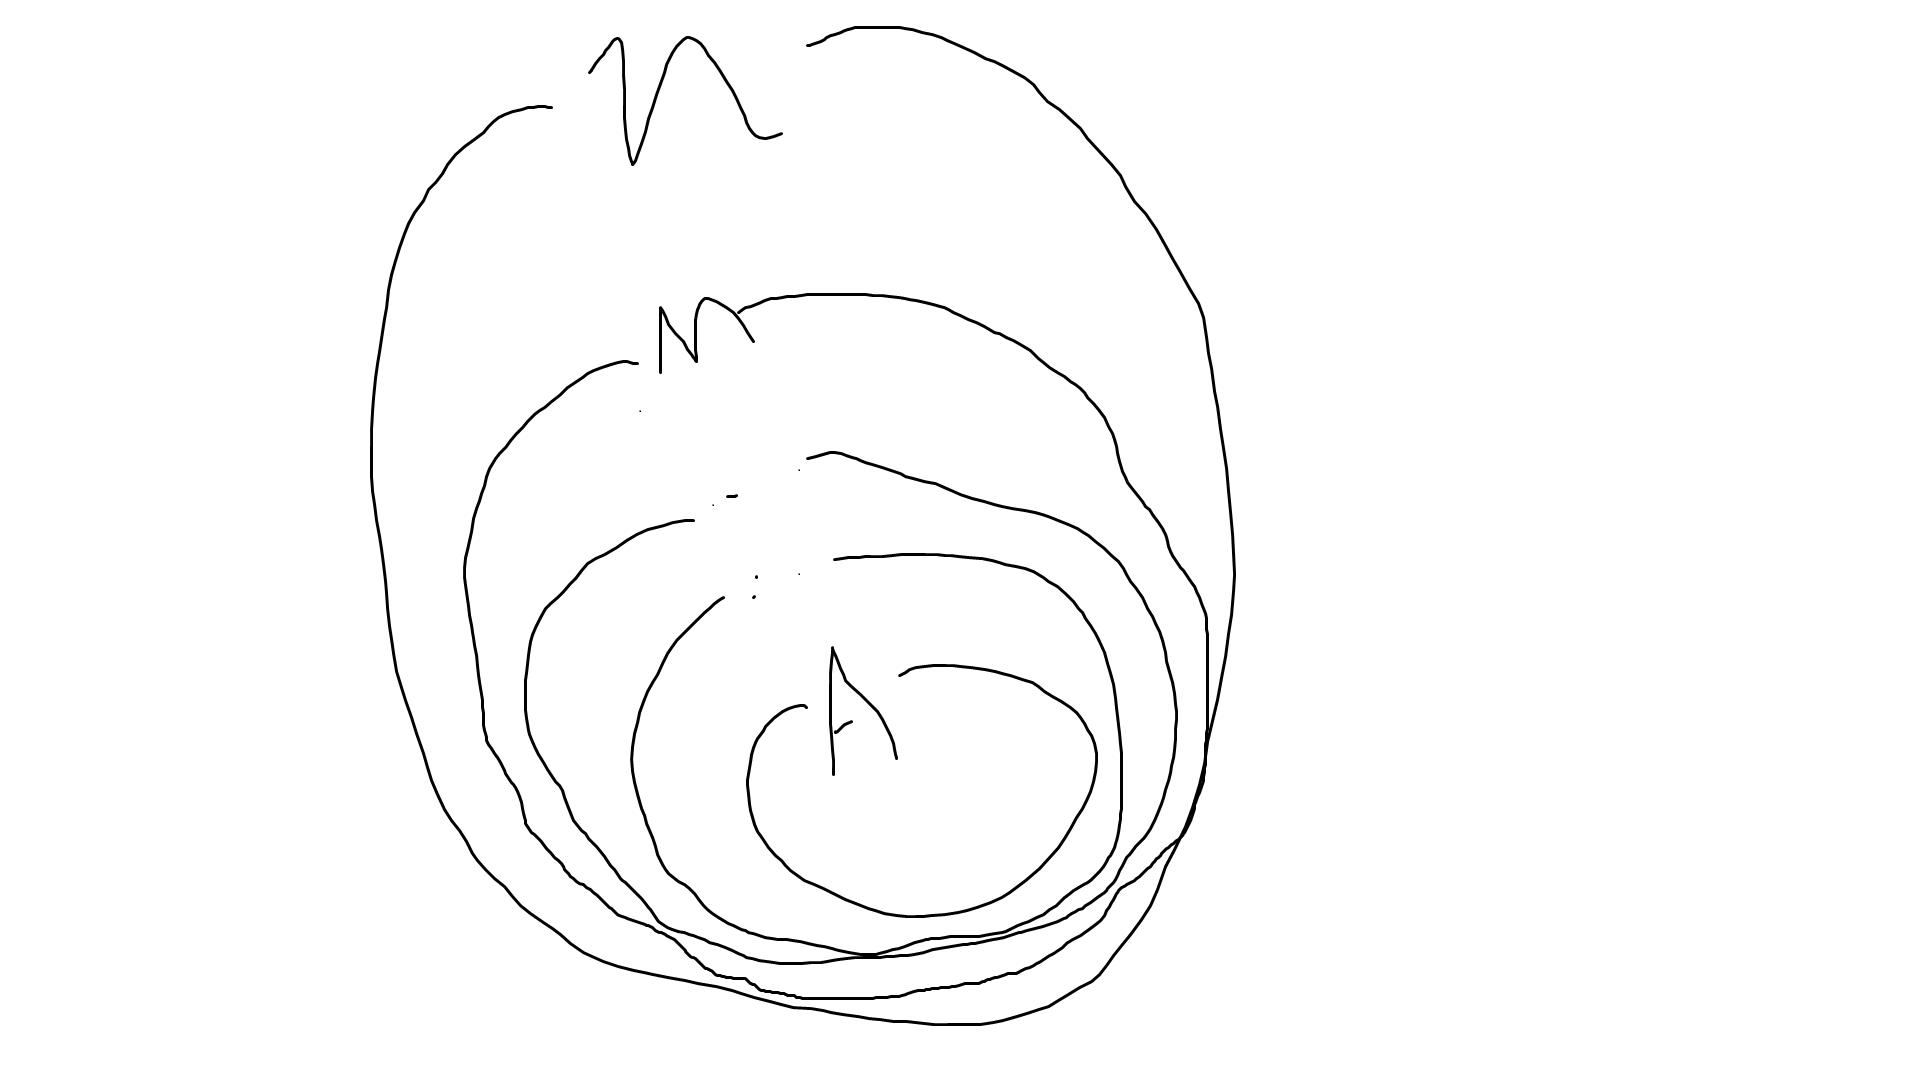
\includegraphics[scale=0.5]{image/Model_02.png}

        Start with $A_0 \subset N$, $A \subseteq A_0$, $|A_0| = l$. The idea is to define $\bra A_i: i <\omega \ket$ so that $M = \cup_{i < \omega}A_i$ satisfies (ii) via the TV test (3.8).\\
        List all formulas $\phi(x,\bar{a})$ ($\bar{a}$ is a tuple in $A_0$), and $\mathcal{N} \vDash \phi(b,\bar{a})$ for some $b$.\\
        Add each such $b$ to $A_0$ (one for each such $\phi$).\\
        Let $A_1 =A_0 \cup \{$ all thes $b$'s$\}$.\\
        Repeat for formulas $\phi(x,\bar{a})$ where $\bar{a}$ is in $A_1$,...\\
        Eventually, $\bra A_i: i<\omega\ket$ is such that $M = \cup_{i < \omega} A_i$ is as required (i.e. $M$ is the domain of some elementary substrucutre of $\mathcal{N}$ that we need).\\
        We claim that $M$ satisfies condition (ii) in Lemma (3.8): Let $\mathcal{N} \vDash \exists x \psi(x,\bar{a})$, where $\bar{a}$ is a tuple in $M$. Then $\bar{a}$ is a \emph{finite} tuple, so there is an $i$ s.t. $\bar{a}$ is in $A_i$.\\
        Then $A_{i+1}$, by construction, contains $b$ s.t. $\mathcal{N} \vDash \phi(b,\bar{a})$. But $A_{i+1} \subseteq M, b \in M$.\\
        Then apply (3.8) we're done.
    \end{proof}
\end{thm}

\newpage

\section{Two relational structures}

\begin{defi} (4.1, dense linear orders)\\
    A \emph{linear order} is an $L_{lo} = \{<\}$-structure such that:\\
    (i) $\forall x \neg (x<x)$;\\
    (ii) $\forall xyz ((x<y \wedge y<z) \to x<z)$;\\
    (iii) $\forall xy((x<y) \vee (y<x) \vee x=y)$ (total).\\
    A linear order is \emph{dense} if, in addition, it also satisfies:\\
    (iv) $\exists xy (x<y)$;\\
    (v) $\forall xy, (x<y \to \exists z (x<z \wedge z<y))$ (density).\\
    A linear order has no endpoints if, in addition, \\
    (vi) $\forall x (\exists y(x<y) \wedge \exists z(z<x))$.\\
    We use $T_{dlo}$ to denote the theory that includes all axioms (i) to (vi), and $T_{lo}$ is the theory that includes axioms (i) to (iii) only.
\end{defi}

\begin{rem}
    (iv) and (v) imply that if $\mathcal{M} \vDash T_{dlo}$, then $|\mathcal{M}| \geq \omega$.
\end{rem}

\begin{defi} (4.2)\\
    If $\mathcal{M},\mathcal{N} \vDash T_{lo}$, then an \emph{injective} map $p:A \subseteq M \to N$ is a \emph{partial embedding} if $\mathcal{M} \vDash a<b \implies \mathcal{N} \vDash p(a) < p(b)$.\\
    In particular, if $|\dom(p)| < \omega$, then $p$ is a \emph{finite} partial embedding.
\end{defi}

\begin{lemma} (4.3, extension lemma)\\
    Take a linear order $\mathcal{M} \vDash T_{lo}$, and a dense linear endpoints $\mathcal{N} \vDash T_{dlo}$, and let $p: M \to N$ be a finite partial embedding. Then if $c \in \mathcal{M}$, there is a finite partial embedding $\hat{p}$ s.t. $p \subseteq \hat{p}$ and $c \in \dom(\hat{p})$.\\
    (\emph{we can always add one extra element in our embedding}.)
    \begin{proof}
        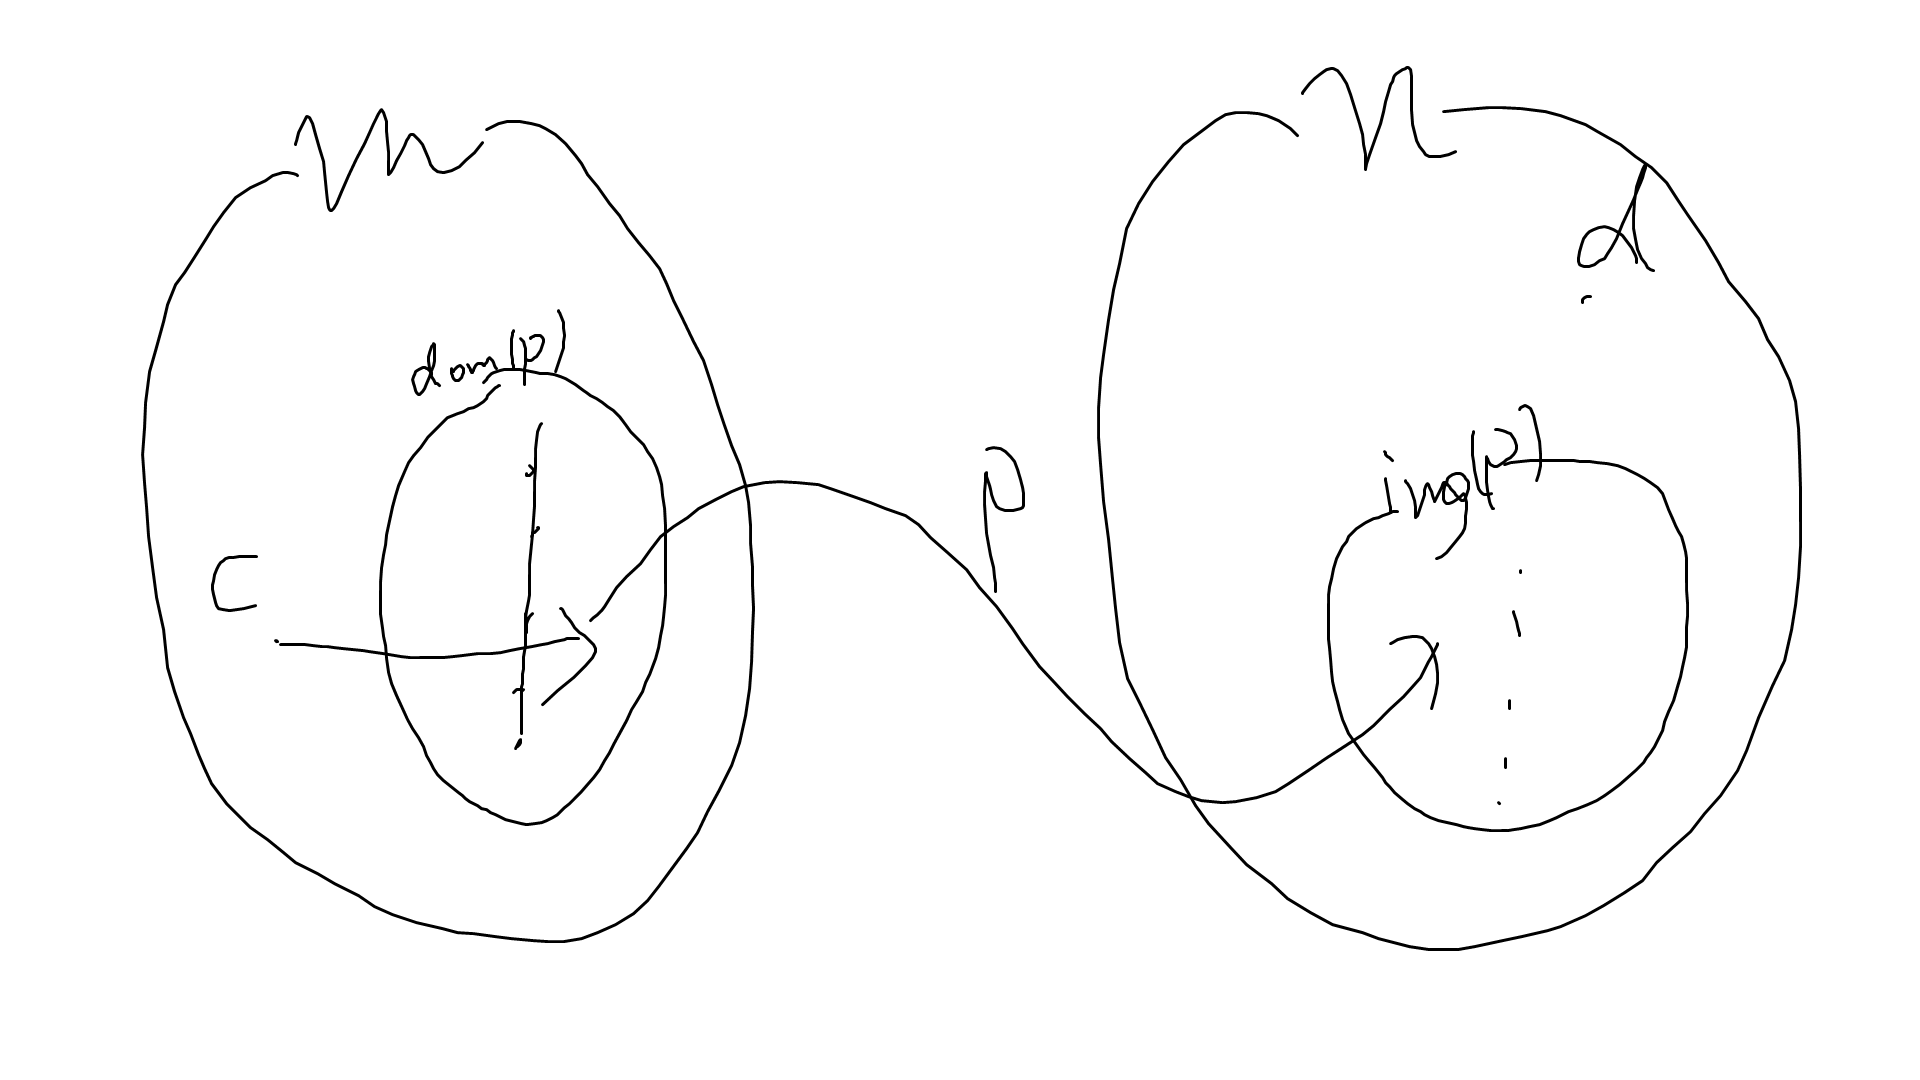
\includegraphics[scale=0.5]{image/Model_03.png}

        Case 1: $c$ is greater than all elements in $\dom(p)$. In that case, pick an element $d \in \mathcal{N}$ s.t. $d>b$ for all $b \in img(p)$;\\
        Case 2: $a_i<c<a_{i+1}$ where $a_i,a_{i+1} \in \dom(p)$. Then we choose $\mathcal{N} \vDash p(a_i) < d < p(a_{i+1})$, where $d$ is chosen appropriately by density (here's the case why we need $\mathcal{N}$ to be dense;\\
        Case 3: $c$ is less than all elements in $\dom(p)$. This is similar to case 1.

        Note that the ability to extend by one point allows us to embed any finite linear order into a dense linear order without endpoints.
    \end{proof}
\end{lemma}

\begin{thm} (4.4)\\
    Let $\mathcal{M},\mathcal{N} \vDash T_{dlo}$ s.t. $|\mathcal{M}| = |\mathcal{N}| = \omega$. Let $p:A \subseteq M \to N$ be a finite partial embedding.\\
    Then there is an isomorphism $\pi:\mathcal{M} \to \mathcal{N}$ s.t. $p \subseteq \pi$.
    \begin{proof}
        Enumerate $M,N$, say $M=\bra a_i:i < \omega\ket$, $N=\bra b_i:i < \omega\ket$ (sequences of elements).\\
        We define, inductively, a chain of finite partial embedding $\bra p_i:i<\omega\ket$ (idea: $\pi = \cup_{i<\omega} p_i$).\\
        Let's start with $p_0 = p$. At stage $i+1$, suppose we are given $p_i$. We want to include $a_i$ in $\dom p_{i+1}$, and $b_i$ in the $img(p_{i+1})$.\\
        (Lecturer calls this a \emph{back and forth} method) Forth step: By lemma 4.3, we can extend $p_i$ to $p_{i+\frac{1}{2}}$ such that $a_i \in \dom(p_{i+\frac{1}{2}})$;\\
        Back step: By lemma 4.3 again applied to $(p_{i+\frac{1}{2}})^{-1}$ to include $b_i \in \dom (p_{i+1}^{-1})$ (i.e. in the range of $p_{i+1}$).\\
        We claim that $p_{i+1}$ extends $p_i$ as required.\\
        Let $\pi = \cup_{i < \omega} p_i$. Then (check) $\pi$ is an isomorphism (i.e. order-preserving bijection).
    \end{proof}
\end{thm}

\begin{defi} (4.5)\\
    An $L$-theory is \emph{consistent} if there is $L$-structure $\mathcal{M}$ s.t. $\mathcal{M} \vDash T$.\\
    If $T$ is a theory in $L$ and $\phi$ is an $L$-sentence, then $T \vdash \phi$ (read as \emph{$T$ entails $\phi$}, note that this has nothing to do with syntactic implication) if for all $\mathcal{M}$ such that $\mathcal{M} \vDash T$, we have $\mathcal{M} \vDash \phi$.\\
    Finally, an $L$-theory $T$ is \emph{complete} if for all $L$-sentences $\phi$, either $T \vdash \phi$ or $T \vdash \neg\phi$ (see part II Logic and Set Theory).\\
    For example, $T_{dlo}$ is complete.
\end{defi}

---Lecture 6---

\begin{defi} (4.6)\\
    A theory $T$ in a countable language with a (infinitely) countable model is \emph{$\omega$-categorical} if any two countable models of $T$ are isomorphic.
\end{defi}

\begin{coro} (4.7 of theorem (4.4))\\
    $T_{dlo}$ is $\omega$-categorical.
    \begin{proof}
        If $\mathcal{M}, \mathcal{N} \vDash T_{dlo}$, $|\mathcal{M}| = |\mathcal{N}| = \omega$, then $\phi$ (the empty map) is a finite partial embedding. But by theorem (4.4) we get $\mathcal{M} \simeq \mathcal{N}$.\\
        (We can also use any $\{\bra a,b\ket\}$ where $a \in \mathcal{M}$ and $b \in \mathcal{M}$ as initial finite partial embedding).
    \end{proof}
\end{coro}

\begin{thm} (4.8)\\
    (erratum 26th Oct 2018: lecturer wants to add a condition \emph{$T$ has no finite models}. Then the problem with (4.11) is fixed.)\\
    If $T$ is an $\omega$-categorical theory in a countable language, then $T$ is complete.
    \begin{proof}
        Let $\mathcal{M} \vDash T$ and $\phi$ be an $L$-sentence.\\
        If $\mathcal{M} \vDash \phi$, suppose $\mathcal{N} \vDash T$. Then by theorem (3.11) (Downward Lowenheim-Skolem), there are $\mathcal{M}' \preccurlyeq \mathcal{M}$, $\mathcal{N}' \preccurlyeq\mathcal{N}$ s.t. $|\mathcal{M}'| = |\mathcal{N}'| = \omega$.\\
        But $\mathcal{M}' \simeq \mathcal{N}'$ (by $\omega$-categoricity), so in particular $\mathcal{M}' \equiv \mathcal{N}'$, and so $\mathcal{N}' \vDash \phi$. By elementarity, $\mathcal{N} \vDash \phi$.\\
        The case $\mathcal{M} \vDash \neg\phi$ is similar.\\
        (Think about if $T$ could have a finite model.)
    \end{proof}
\end{thm}

\begin{coro} (4.9)\\
    $T_{dlo}$ is complete.
\end{coro}

\begin{defi} (4.10)\\
    If $\mathcal{M}$, $\mathcal{N}$ are $L$-structures, a map $f$ such that $\dom (f) \subseteq M$ (the domain of $\mathcal{M}$), and $img(f) \subseteq N$ is a (partial) \emph{elementary map} if for all $L$-formulas $\phi(\bar{x})$ and $\bar{a} \in (\dom(f))^{|\bar{x}|}$, then
    $$\mathcal{M} \vDash \phi(\bar{a}) \iff \mathcal{N} \vDash \phi(f(\bar{a}))$$
\end{defi}

\begin{rem} (4.11)\\
    A map $f$ is elementary iff every finite restriction of $f$ is elementary.\\
    (Why? For forward, if $f_0 \subseteq f$ is a finite restriction that is not elementary, then for some formula $\phi(\bar{x})$, $\bar{a} \in \dom (f_0)$, the above equivalence doesn't hold; but then that equivalence doesn't hold for $f$ either; contradiction; for backward, if $f$ is not elementary, then the above equivalence fails on a finite tuple, so the above equivalence fails on some finite restriction.)
\end{rem}

\begin{prop} (4.12)\\
    Let $\mathcal{M},\mathcal{N} \vDash T_{dlo}$, and let $p: A \subseteq M \to N$ be a partial embedding. Then $p$ is elementary.\\
    \begin{proof}
        By remark (4.11), it suffices to consider $p$ finite.\\
        By Downward L-S theoem (3.11), we choose $\mathcal{M}',\mathcal{N}'$ such that\\
        (i) $|\mathcal{M}'| = |\mathcal{N}'| = \omega$;\\
        (ii) $\mathcal{M}' \preccurlyeq\mathcal{M}$, $\mathcal{N}' \preccurlyeq\mathcal{N}$;\\
        (iii) $\dom (p) \subseteq M', img(p) \subseteq N'$.

        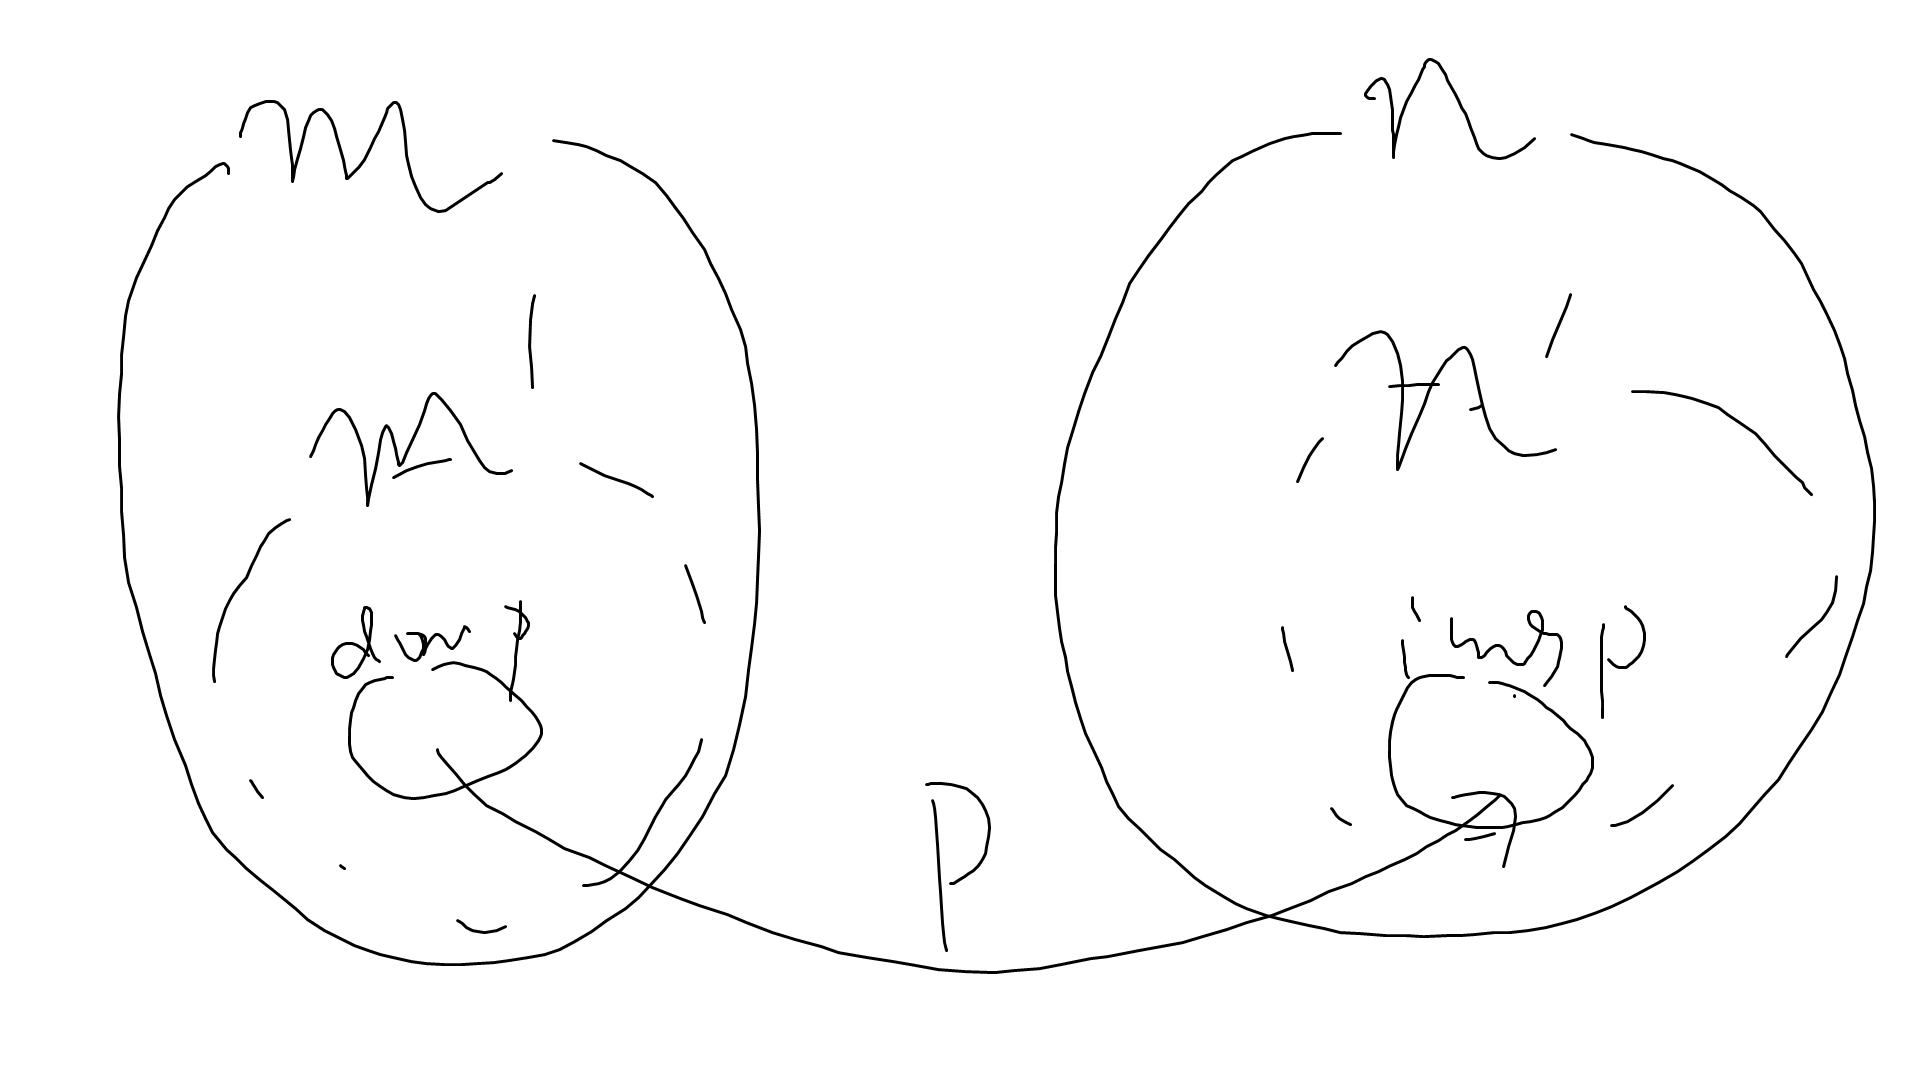
\includegraphics[scale=0.5]{image/Model_04.png}

        Now $p$ is a finite partial embedding between countable models, so $p$ extends to an isomorphism $\pi:\mathcal{M}' \to \mathcal{N}'$.\\
        In particular, $\pi$ is an elemntary map between $\mathcal{M}$ and $\mathcal{N}$.
    \end{proof}
\end{prop}

\begin{coro} (4.13)\\
    $(\Q,<) \preccurlyeq (\R,<)$.\\
    \begin{proof}
        Use proposition (4.12) with $id:\Q \to \R$.
    \end{proof}
\end{coro}

\begin{defi} (4.14)\\
    (See Part II Logic and Set Theory)\\
    Let $L_{gph} = \{R\}$, where $R$ is a binary relation symbol.\\
    An $L_{gph}$-structure is a graph if\\
    (i) $\forall x$ $\neg R(x,x)$;\\
    (ii) $\forall xy (R(x,y) \leftrightarrow R(y,x))$.

    An $L_{gph}$-structure is a \href{http://modeltheory.wikia.com/wiki/Random_graph}{random graph} if it is a graph such that the following axiom-schema $(r_n)$ hold:

    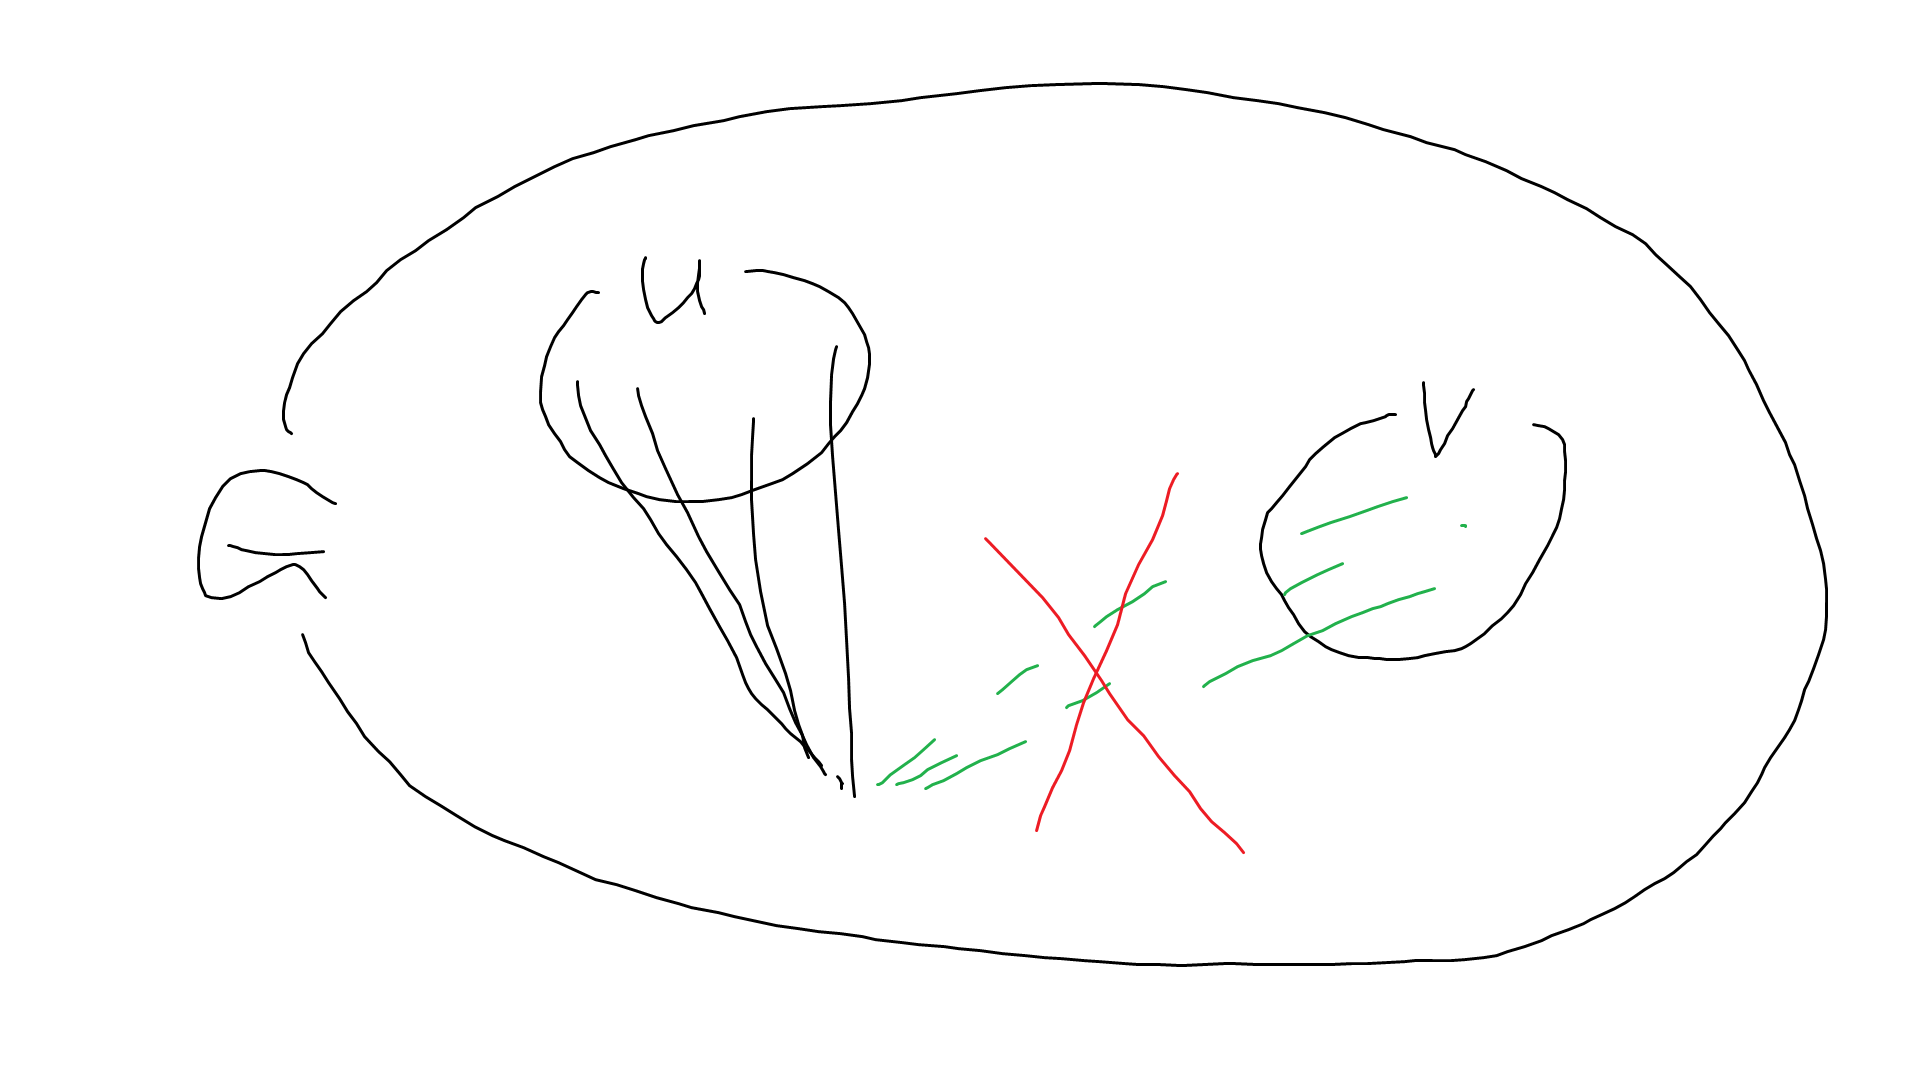
\includegraphics[scale=0.5]{image/Model_05.png}

    $$\forall x_0...x_n,y_0...y_n, (\bigwedge_{i,j=0}^n x_i \neq y_j \to \exists z(\bigwedge_{i = 0}^n (z \neq x_i) \wedge (z \neq y_i) \wedge R(z,x_i) \wedge \neg R(z,y_i)))$$

    (iii) $\exists xy (x\neq y)$.
\end{defi}

\begin{rem} (similar to what is mentioned in the link above)\\
    A random graph is infinite. Given a finite subset, we can always find a vertex that is connected to every vertex in the subset (likewise for not connected).
\end{rem}

\begin{fact} (4.15)\\
    There is a random graph.
    \begin{proof}
        Let the domain be $\omega$, let $i,j \in \omega$ such that $i < j$. Write $j$ as a sum of distinct powers of $2$. Then $\{i,j\}$ is an edge iff $2^i$ appears in the sum.\\
        As an exercise, prove that $\omega$ with this definition of $R$ is indeed a random graph.
    \end{proof}
\end{fact}

\begin{defi} (4.16, or more precisely just notations)\\
    $T_{gph} = \{$axioms (i), (ii)$\}$, $T_{rg} = T_{gph} \cup \{$(iii), ($r_n$) $:n \in \omega\}$.\\
    If $\mathcal{M},\mathcal{N} \vDash T_{gph}$, a partial embedding is an injection $p: A \subseteq M \to N$ s.t. $\mathcal{M} \vDash R(p(a),p(b)) \iff \mathcal{N} \vDash R(a,b)$ for all $a,b$ in the domain.
\end{defi}

\begin{lemma} (4.17)\\
    Let $\mathcal{M} \vDash T_{gph},\mathcal{N} \vDash T_{rg}$, let $p:A \subseteq M \to N$ be a finite partial embedding, and let $c \in M$.\\
    Then there is a map $\hat{p}:\hat{A} \subseteq M \to N$ such that $\hat{p}$ is a partial embedding, $c \in \dom \hat{p}$, $p\subseteq \hat{p}$.\\
    (This is like another extension lemma.)\\
    We'll prove this next time.
    
    ---Lecture 7---

    Last time we defined what a random graph is (in this course). We also defined what is a partial embedding in this theory (just preserves all edges).\\
    Let's continue with the proof of the lemma now. Let $c \in M$, $c \not\in \dom(p)$.

    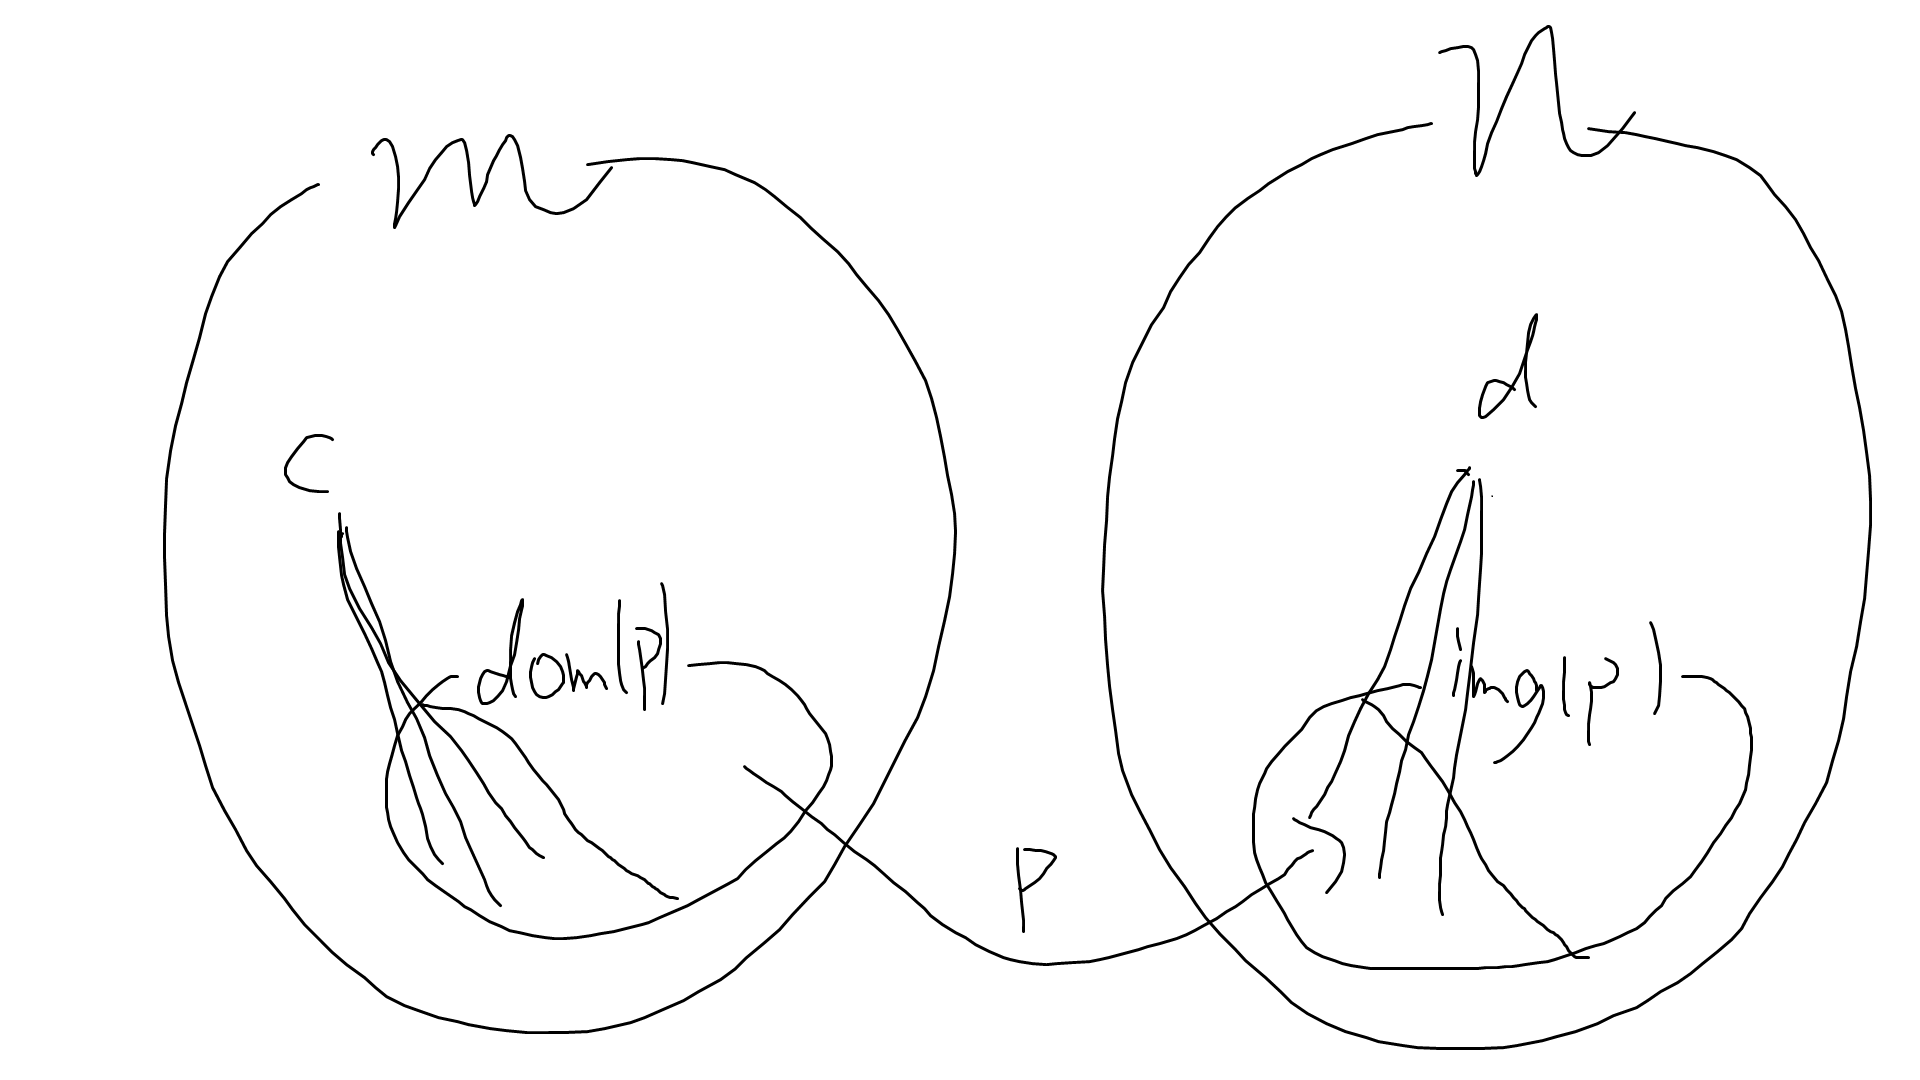
\includegraphics[scale=0.5]{image/Model_06.png}

    Find $d \in N$ such that $\mathcal{N} \vDash R(d,p(a)) \iff \mathcal{M} \vDash R(c,a)$.
\end{lemma}

\begin{thm} (4.18)\\
    Let $\mathcal{M},\mathcal{N} \vDash T_{rg}$ and $|\mathcal{M}| = |\mathcal{N}| = \omega$, and $P:A \subseteq M \to N$ is a finite partial embedding.\\
    Then $\mathcal{M} \simeq \mathcal{N}$, by an isomorphism that extends $p$.
    \begin{proof}
        Same as proof of Theorem (4.4) (there is only one model of $T_{dlo}$ up to isomorphism), but with lemma (4.17) instead of lemma (4.3).
    \end{proof}
\end{thm}

\begin{coro} (4.19)\\
    $T_{rg}$ is $\omega$-categorical (see definition (4.6) -- this is just a restatement of the theorem above) and complete.\\
    In particular, every finite partial embedding between models of $T_{rg}$ is an elementary map.
\end{coro}

\begin{rem}
    The unique (up to isomorphism) model of $T_{rg}$ is \emph{the} countable random graph, or the \emph{Rado} graph.\\
    It is universal w.r.t. finite and countable graphs (i.e. it embeds all).\\
    Another nice property (which you are not required to see this immediately -- it is far from trivial) \emph{ultrahomogeneous}, i.e. every isomorphism between finite substructures extends to an automorphism of the whole graph.\\
    Google \emph{David Marker's} book, or \emph{Tent-Ziegler}. Warning: both of them contain a lot of typos.
\end{rem}

\newpage

\section{Compactness}

\begin{defi} (5.1)\\
    Suppose we have a $L$-theory $T$.\\
    (i) $T$ is \emph{finitely satisfiable} if every finite subset of sentences in $T$ has a model.\\
    (ii) $T$ is \emph{maximal} if for all $L$-sentences $\sigma$, either $\sigma \in T$ or $\neg\sigma \in T$.\\
    (iii) $T$ has the \emph{witness property} (WP): if for all $\phi(x)$ ($L$-formula with $1$ free variable), there is a constant $c \in \mathcal{C}$ s.t.
    $$(\exists x \phi(x) \to \phi(c)) \in T$$
\end{defi}

\begin{lemma} (5.2)\\
    If $T$ is maximal and finitely satisfiable (we'll sometimes use \emph{f.s.} from now onwards), and $\phi$ is an $L$-sentence, and $\triangle \stackrel{fin}{\subseteq} T$ and $\triangle \vdash \phi$, then $\phi \in T$.\\
    (Prove it by yourself)
\end{lemma}

\begin{lemma} (5.3)\\
    Let $T$ be a maximal, f.s. theory with WP. Then $T$ has a model.\\
    Moreover, if $\lambda$ is a cardinal and $|\mathcal{C}| \leq L$ ($\mathcal{C}$ is the set of constants in $L$), then $T$ has a model of size at most $\lambda$.
    \begin{proof}
        Let $\mathcal{C}$ be the constants of $L$. Let $c,d \in \mathcal{C}$, define $c \sim d$ iff $c=d \in T$.\\
        We claim that $\sim$ is an equivalence relation: reflexivity and symmetry are trivial; for transitivity, let $c \sim d$ and $d \sim e$. Then $c=d \in T$ and $d=e \in T$. Then by the lemma $c=e\in T$ as it is implied by the two sentences. So $c \sim e$.\\
        Notation: we'll use $c/\sim = c^*$ to denote the equivalence class of $c$.\\
        Now define a structure $\mathcal{M}$ whose domain is $\mathcal{C}/\sim = M$. Clearly, $|M| \leq \lambda$ if $|\mathcal{C}| \leq \lambda$.\\
        We must define interpretations in $\mathcal{M}$ for symbols for $L$:\\
        $\bullet$ If $c \in \mathcal{C}$, then $c^m = c^* (=c/\sim$);\\
        $\bullet$ If $R \in \mathcal{R}$ is a relation symbol, we define $R^{\mathcal{M}} = \{(c_1^*,...,c_{n_R}^*):R(c_1,...,c_{n_R}) \in T\}$.\\
        We have to check that $R^{\mathcal{M}}$ is well-defined: suppose $\bar{c},\bar{d} \in \mathcal{C}^{n_R}$ and suppose $c_i \sim d_i$ for each $i$, i.e. $c_i = d_i \in T$ for every $i=1,...,n_R$. However, now
        $$R(\bar{c}) \in T \iff R(\bar{d}) \in T$$
        by maximality of $T$ and the previous lemma. So that $R^{\mathcal{M}}$ is well defined.\\
        $\bullet$ If $f \in \mathcal{F}$ is a function symbol, then $f\bar{c} = d \in T$ for some $d \in \mathcal{C}$: this is because $\exists x(f(\bar{c}=x) \in T$ by maximality and f.s..\\
        Then define $f^{\mathcal{M}}(\bar{c}^*) = \bar{d}^*$ (obvious notation).\\
        We also have to check this is well-defined. Lecturer decides to left this to us.\\
        Now we claim that the terms behave nicely as what the theory says, i.e. if $t(x_1,...,x_n)$ is an $L$-term and $c_1,...,c_n,d \in \mathcal{C}$, then $t(c_1,...,c_n) = d \in T \iff t^{\mathcal{M}} (c_1^*,...,c_n^*) = d^*$.\\
        $\bullet$ $\implies$: by induction on the complexity of $T$ (lecturer decided to leave this as another exercise).\\
        $\bullet$ $\Leftarrow$: Assume $t^{\mathcal{M}} (c_1^*,...,c_n^*) = d^*$. Then $t(c_1,...,c_n) = e \in T$ for some constant $e$ (why? As our theory is maximal, it has to say what the result is when we apply $t$ to these terms). We then use $\implies$ to get that $t^{\mathcal{M}}(c_1^*,...,c_n^*) = e^*$.\\
        But then $d^* = e^*$, i.e. $d = e \in T$. So by lemma (5.2), the sentence implied by these two sentences, $t(c_1,...,c_n) = d \in T$.\\
        The last massive claim: for all $L$-formulas $\phi(\bar{x})$ and $\bar{c} \in \mathcal{C}^{|\bar{x}|}$, we have
        $$\mathcal{M} \vDash \phi(\bar{c}) \iff \phi(\bar{c}) \in T$$
        The proof is by induction on complexity of $\phi(\bar{x})$ (The lecturer decided to leave yet another proof to us -- lots of work to be done here. Lecturer is speeding up!).
    \end{proof}
\end{lemma}

\end{document}
